%%%%%%%%%%%%%%%%%%%%%%%%%%%%%%%%%%%%%%%%%%%%%%%%%%%%%%%%%%%%%%%%%
% Contents : The budget chapter
% $Id : grisbi-manuel-budget.tex, v 0.8.9 2012/04/27 Jean-Luc Duflot
% $Id : grisbi-manuel-budget.tex, v 1.0 2014/02/12 Jean-Luc Duflot
%%%%%%%%%%%%%%%%%%%%%%%%%%%%%%%%%%%%%%%%%%%%%%%%%%%%%%%%%%%%%%%%%

\chapter{Budgets prévisionnels\label{budget}}


Un budget est un document récapitulatif des recettes et des dépenses prévisionnelles pour un agent économique (individu, ménage, entreprise, État, etc.) pour un exercice comptable à venir.

Grisbi vous permet de définir, pour chaque compte, un budget prévisionnel par exercice ou sur douze mois, basé sur les données historiques précédentes classées suivant leurs imputations budgétaires ou leurs imputations comptables (catégories et sous-catégories). Au moment de son établissement, un budget n'a de valeur que si les \indexword{prévisions}\index{prévision} affichées sont conformes à la réalité qu'elles sont censées décrire  : aucune dépense ne doit être \og oubliée \fg{} ou minorée, aucun revenu ne doit être majoré\ldots

Grisbi vous permet aussi de faire un suivi de vos \indexword{emprunts}\index{emprunt} à travers les \indexword{comptes de passif}\index{compte !passif}, en créant des tableaux d'amortissement.

% espace pour changement de thème
\vspacepdf{5mm}
Pour avoir accès au budget prévisionnel ou au tableau d'amortissement pour un compte, sélectionnez ce compte dans le panneau de navigation ou avec la barre d'information (voir le chapitre \vref{home}, \menu{Accueil}) : le panneau de navigation affiche le nom du compte sur fond bleu{\couleur}, et le pavé des détails affiche tous les onglets disponibles du compte. 

Si le compte sélectionné n'a pas encore été configuré pour un budget prévisionnel ou un tableau d'amortissement, seuls les onglets \menu{Opérations} et \menu{Propriétés} sont affichés : dans ce cas, suivez la procédure \menu{Création d'un budget prévisionnel}, pour un compte de banque ou de caisse (voir la section \vref{budget-create}), ou bien \menu{Création d'un tableau d'amortissement}, pour un compte de passif (voir la section \vref{budget-amortizationCreate}).

Sinon, si le compte sélectionné a été auparavant configuré pour un budget prévisionnel ou un tableau d'amortissement, le pavé des détails affiche d'autres onglets, suivant le type du compte :

\begin{itemize}
	 \item pour les comptes de banque ou de caisse :
		\begin{itemize}
			 \item \menu{Prévisions},
			 \item \menu{Données historiques} ;

\textbf{Note} : pour les comptes de caisse, l'onglet \menu{Prévisions} n'est affiché  que si l'on a choisi d'afficher aussi leurs prévisions.
		\end{itemize}
	 \item pour les comptes de passif :
		\begin{itemize}
			 \item \menu{Tableau d'amortissement}.
		\end{itemize}
\end{itemize}

% espace avant Attention ou Note  : 5 mm
\vspacepdf{5mm}
\textbf{Note} : il est vivement conseillé de consulter les sections suivantes décrivant ces différents onglets, avant de commencer l'établissement de budgets prévisionnels ou de tableaux d'amortissement.


\section{Données historiques\label{budget-data}}


L'onglet \menu{Données historiques} contient l'ensemble des données qui vont servir de base à l'établissement de votre \indexword{prévision}\index{prévision}. Ce sont toutes les opérations déjà enregistrées dans votre compte, relatives à une période de temps donnée, et groupées en catégories ou imputations budgétaires.

% espace pour changement de thème
\vspacepdf{5mm}
Pour afficher les détails des \menu{Données historiques}, sélectionnez leur onglet. Il affiche trois \ifIllustration éléments\refimage{budget-historicalData-img} :
\else éléments : 
\fi

\begin{itemize}
	\item la barre d'outils ;
	\item l'en-tête des données historiques ; 
	\item le tableau des données historiques.
\end{itemize}

\ifIllustration
% image centrée
\begin{figure}[htbp]
\begin{center}
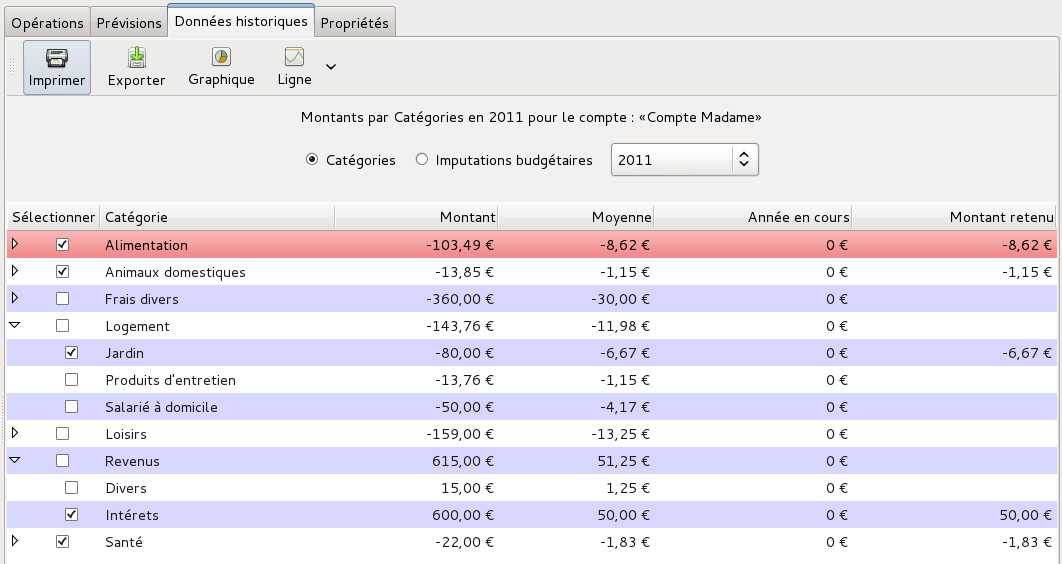
\includegraphics[scale=0.5]{image/screenshot/budget_historical_data}
\end{center}
\caption{Onglet des données historiques}
\label{budget-historicalData-img}
\end{figure}
% image centrée
\fi


\subsection{Barre d'outils\label{budget-data-functions}}

La barre d'outils présente les fonctions suivantes : 
\begin{itemize}
	 \item \menu{Imprimer} : ouvre la fenêtre de sélection de l'imprimante et de ses options ;
	 \item \menu{Exporter} : permet d'exporter le tableau des prévisions dans un fichier ;
	 \item \menu{Graphique} : affiche deux graphiques en secteurs, pour les revenus et les dépenses ;
	 \item \menu{Ligne} ou \menu{Colonne} : affiche un graphique temporel, pour l'évolution du montant d'une ligne dans le tableau ;
	 \item une liste déroulante : permet de choisir le graphique par défaut \menu{Ligne} ou \menu{Colonne}.	 
\end{itemize}

\ifIllustration
% saut de page pour titre solidaire
\newpage
\fi

\subsection{En-tête des données historiques\label{budget-data-source}}

L'en-tête des données historiques s'affiche en haut du pavé des détails. Il affiche les paramètres nécessaires pour établir les prévisions,  tels qu'ils auront été définis auparavant, en particulier dans le menu \menu{Édition - Préférences} (voir la section \vref{setup-budget-data}, \menu{Données des comptes}). Ces paramètres sont les suivants :

\begin{itemize}
	\item le \indexword{titre des données historiques}\index{titre !données historiques} : \menu{Montants par \ldots{ } sur \ldots{ } pour le compte\ldots}{ }, suivi du nom du compte ;
	\item l'origine des \indexword{données de référence}\index{données de référence} : soit les  \menu{Catégories}, soit les \menu{Imputations budgétaires} ;
	\item la \indexword{période de référence}\index{période de référence} : soit un exercice, soit \menu{12 mois glissants}.
	% espace pour note à la ligne suivante

	\textbf{Note} : le choix des exercices ne s'affiche que si au moins un exercice a été défini (voir la section \vref{financialyear-start}, \menu{Mise en place des exercices}).
\end{itemize}


\subsection{Tableau des données historiques\label{budget-data-table}}

Le tableau des données historiques s'affiche en bas du pavé des détails, sous l'en-tête des données historiques. Il affiche toutes les opérations déjà enregistrées dans le compte et appartenant à la période de référence, qui vont servir à établir la prévision.

% espace pour changement de thème
\vspacepdf{5mm}
Ce tableau affiche en haut la barre de libellés des colonnes. Vous pouvez \indexword{élargir ou rétrécir une colonne}\index{colonne !largeur} en cliquant sur le séparateur entre deux colonnes et en le déplaçant. Vous pouvez déplacer le tableau vers le haut ou vers le bas avec la molette de la souris, ou bien avec la souris et l'ascenseur vertical. 

%XXXXXX Ne fonctionne pas  : XXXXXX Pour rétablir la largeur des colonnes à leur valeur par défaut, sélectionnez le menu \menu{Affichage - Réinitialiser la largeur des colonnes}. XXXXXX Ne fonctionne pas  : XXXXXX

Il affiche autant de lignes qu'il y a dans le compte de catégories et de sous-catégories, ou bien d'imputations budgétaires et de sous-imputations budgétaires. Ses champs d'affichage sont les suivants :
\begin{itemize}
	\item\menu{Sélectionner} : permet, en cliquant sur le petit triangle noir, de \indexword{dérouler ou d'enrouler les sous-catégories}\index{sous-catégories !déroulées} (ou sous-imputations budgétaires\index{sous-imputations budgétaires !déroulées}) éventuelles, et en cliquant dans les cases, de sélectionner une ligne ; 

	\textbf{Note} : ces triangles peuvent être remplacés, en fonction du thème de l'environnement de bureau ou du gestionnaire de fenêtres que vous utilisez, par d'autres caractères tels que +, -, >, <, etc.
	
	\item \menu{Catégories} ou \menu{Imputations budgétaires} : (sous-) catégories ou (sous-) imputations budgétaires concernées ;
	\item \menu{Montant} : total des montants des opérations d'une (sous-) catégorie ou d'une (sous-) imputation budgétaire sur la période ;
	\item \menu{Moyenne} : moyenne mensuelle des montants des opérations d'une (sous-) catégorie ou d'une (sous-) imputation budgétaire sur la période ;
	\item \menu{Année en cours} : total des montants des opérations déjà effectuées dans l'année ou l'exercice en cours, pour une (sous-) catégorie ou une (sous-) imputation budgétaire ;
	\item \menu{Montant retenu } : \indexword{montant retenu}\index{montant !retenu} pour la prévision ; il est soit déterminé par votre choix dans le menu contextuel de la ligne, soit saisi par vous-même manuellement dans ce champ. Ce montant est reporté dans la prévision, au dernier jour du mois.
\end{itemize}
 

%XXXXXX Ne fonctionne pas  : XXXXXX
%Le déplacement vers la gauche ou la droite se fait avec la souris et l'ascenseur horizontal. XXXXXX Ne fonctionne pas  : XXXXXX

% espace pour changement de thème
\vspacepdf{5mm}
Chaque (sous-) catégorie ou (sous-) imputation budgétaire est affichée sur une seule ligne. Pour une bonne lisibilité de l'affichage, Grisbi présente une alternance de couleurs de fond violet et blanc{\couleurs} à chaque ligne.

% espace pour changement de thème
\vspacepdf{5mm}
Pour sélectionner une (sous-) catégorie ou une (sous-) imputation budgétaire, vous avez deux moyens :
\begin{itemize}
	 \item cliquer sur sa ligne ;
	 \item déplacer la sélection avec les touches du clavier \key{Flèche Haut}, \key{Flèche Bas}, \key{Page Haut}et \key{Page Bas}.
\end{itemize}
La ligne apparaît alors sur fond rouge{\couleur}.

% espace pour changement de thème
\vspacepdf{5mm}
Un menu contextuel est disponible par un clic-droit sur une ligne, et propose les actions suivantes :
\begin{itemize}
	\item \menu{Assigner le montant de la dernière opération} : copie  le montant de la dernière opération de la (sous-) catégorie ou (sous-) imputation budgétaire dans le champ \menu{Montant retenu} ;
	\item \menu{Copier la valeur moyenne} : copie la valeur moyenne sur la période de toutes les opérations de la (sous-) catégorie ou (sous-) imputation budgétaire dans le champ \menu{Montant retenu}.
	% espace pour note à la ligne suivante

	\textbf{Note} : si vous sélectionnez ce choix pour une ligne non mensuelle, son montant sera reporté chaque mois dans les prévisions, qui seront donc faussées.
\end{itemize}


\subsection{Graphiques sur les données historiques\label{budget-data-chart}}

Pour afficher les \indexword{graphiques sur les données historiques}\index{données historiques !graphiques} d'un compte, vous disposez de trois outils dans la barre d'outils : 

\begin{itemize}
	 \item \menu{Graphique} : affiche deux graphiques en secteurs, pour les revenus et les dépenses ;
	 \item \menu{Ligne} ou \menu{Colonne} : affiche un graphique temporel, pour l'historique d'évolution du montant d'une ligne du tableau ;
	 \item une liste déroulante : permet de choisir le graphique par défaut \menu{Ligne} ou \menu{Colonne}.
\end{itemize}


\subsubsection{Graphiques en secteurs}

Pour afficher les graphiques en secteurs, cliquez sur l'outil \menu{Graphique} dans la barre d'outils. Une fenêtre affiche, sous la forme de deux graphiques en secteurs, pour les revenus et les dépenses, l'ensemble des montants sélectionnés dans le tableau des données historiques, par catégories ou imputations budgétaires selon le cas, et sur la période de référence : soit un exercice, soit \menu{12 mois glissants}.

\textbf{Note} : le choix des exercices ne s'affiche que si au moins un exercice a été défini (voir la section \vref{financialyear-start}, \menu{Mise en place des exercices}).

Le placement du pointeur de souris au-dessus d'un secteur affiche dans une info-bulle son nom, son montant et son pourcentage par rapport au total du secteur, et un clic-droit dessus affiche un autre graphique en secteur relatif à ses sous-catégories ou sous-imputations budgétaires, s'il y a lieu.

Ces graphiques fournissent une représentation visuelle des rapports entre les différents postes de dépenses ou de revenus passés, et permettent d'affiner votre sélection de données, par exemple en ne sélectionnant que les plus importantes.


\subsubsection{Graphiques temporels}

L'outil \menu{Ligne} ou \menu{Colonne} sert de choix par défaut, et la liste déroulante à sa droite permet de changer ce choix par défaut, donc de remplacer l'outil \menu{Ligne} par l'outil \menu{Colonne} et inversement.

Ces deux graphiques fournissent une représentation visuelle de l'évolution passée du montant \menu{Année en cours} d'une ligne du tableau des données historiques, et permettent d'en anticiper les conséquences par des mesures appropriées.

\paragraph{Graphique temporel en ligne :} pour afficher ce graphique, sélectionnez une des lignes de (sous-) catégorie ou de (sous-) imputation budgétaire dans le tableau des données historiques, puis cliquez dans la barre d'outils sur l'outil \menu{Ligne} ou sur le libellé \menu{Ligne} de la liste déroulante ; une fenêtre affiche, dans son onglet \menu{Graphique}, le nom et le montant pour l'\menu{Année en cours} de la ligne sélectionnée, et sa courbe d'évolution sur la période de référence. Vous pouvez afficher des lignes de niveau en cliquant sur le bouton \menu{Montrer la grille}, et les enlever par le bouton \menu{Cacher la grille}. 

Vous pouvez définir, dans l'onglet \menu{Options}, la présentation du graphique pour l'axe horizontal (graduation principale, position, ligne supplémentaire, orientation) et pour l'axe vertical (grille principale et secondaire). 

\paragraph{Graphique temporel en colonne :} pour afficher ce graphique, sélectionnez une des lignes de (sous-) catégorie ou de (sous-) imputation budgétaire dans le tableau des données historiques, puis cliquez dans la barre d'outils sur l'outil \menu{Colonne} ou sur le libellé \menu{Colonne} de la liste déroulante ; une fenêtre affiche, dans son onglet \menu{Graphique}, le nom et le montant pour l'\menu{Année en cours} de la ligne sélectionnée, et son évolution sur la période de référence, sous la forme de barres verticales. Vous pouvez afficher des lignes de niveau en cliquant sur le bouton \menu{Montrer la grille}, et les enlever par le bouton \menu{Cacher la grille}.

Vous pouvez définir, dans l'onglet \menu{Options}, la présentation du graphique pour l'axe horizontal (graduation principale, position, ligne supplémentaire, orientation) et pour l'axe vertical (grille principale et secondaire), ainsi que pour les barres (espacement et superposition de la grille).


\section{Prévisions\label{budget-estimate}}


L'onglet \menu{Prévisions} contient l'ensemble des résultats calculés à partir des choix de configuration et du tableau des données historiques.

% espace pour changement de thème
\vspacepdf{5mm}
Pour afficher les détails des \menu{Prévisions}, sélectionnez son onglet. Il affiche trois \ifIllustration éléments\refimage{budget-estimate-img} :
\else éléments : 
\fi

\begin{itemize}
	\item la barre d'outils ;
	\item l'en-tête des prévisions ; 
	\item le tableau des prévisions.
\end{itemize}

\ifIllustration
% image centrée
\begin{figure}[t]
\begin{center}
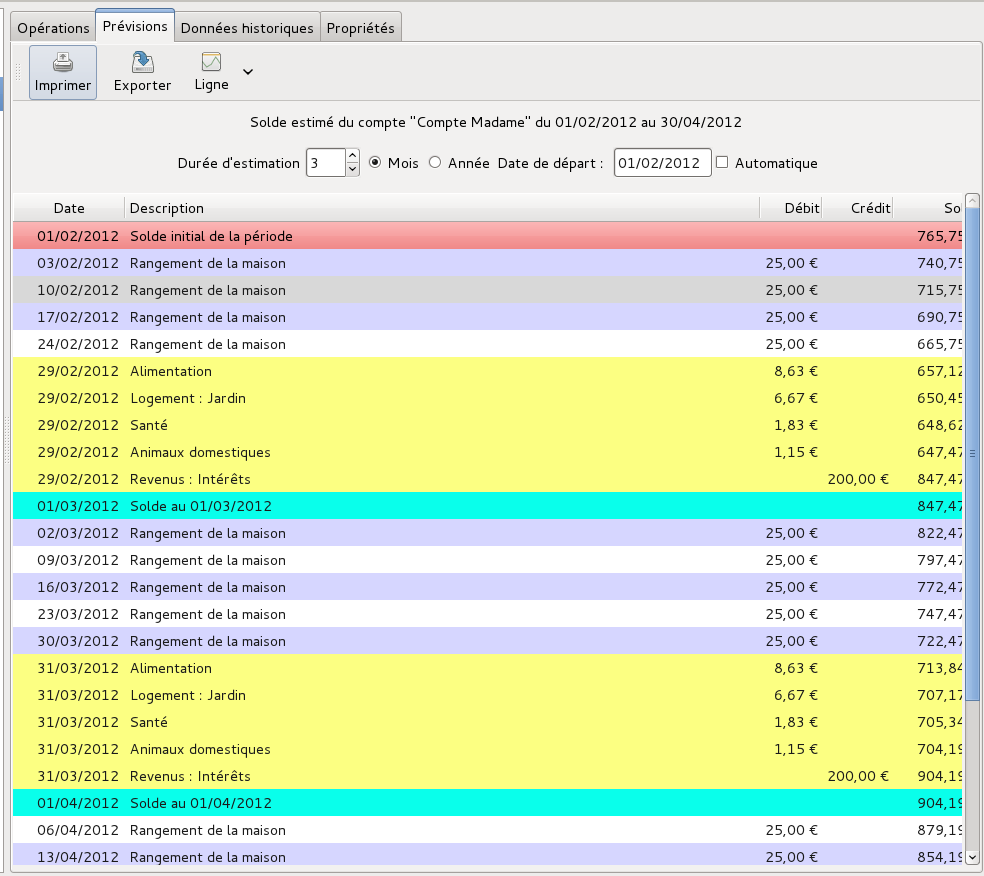
\includegraphics[scale=0.49]{image/screenshot/budget_estimate}
\end{center}
\caption{Onglet des prévisions}
\label{budget-estimate-img}
\end{figure}
% image centrée
\fi

\ifIllustration
\else
% saut de page pour titre solidaire
\newpage
\fi

\subsection{Barre d'outils\label{budget-estimate-functions}}

La barre d'outils présente les fonctions suivantes  : 
\begin{itemize}
	 \item \menu{Imprimer} : ouvre la fenêtre de sélection de l'imprimante et de ses options ;
	 \item \menu{Exporter} : permet d'exporter le tableau des prévisions dans un fichier ;
	 \item \menu{Ligne} ou \menu{Colonne} : affiche un graphique temporel, pour l'évolution du montant du solde du compte ;
	 \item une liste déroulante : permet de choisir le graphique par défaut \menu{Ligne} ou \menu{Colonne}.	 
\end{itemize}


\subsection{En-tête des prévisions\label{budget-estimate-summary}}

L'en-tête des prévisions s'affiche en haut du pavé des détails, sous la barre d'outils. Il affiche les paramètres tels qu'ils ont été définis auparavant, en particulier dans le menu \menu{Édition - Préférences} (voir la section \vref{setup-budget-data}, \menu{Données des comptes}). Ces paramètres sont les suivants :
\begin{itemize}
	\item le \indexword{titre de la prévision}\index{titre !prévision}  : \menu{Solde estimé du compte\ldots{ }}\index{solde !estimé}, suivi du nom du compte et de la période de prévision ;
	\item \menu{Durée d'estimation} : la \indexword{durée d'estimation}\index{durée !estimation} est la période de temps sur laquelle les prévisions sont données, en nombre de mois ou d'années ; elle est au maximum de 5 ans ;
	\item \menu{Date de départ de l'estimation} : la \indexword{date de départ de l'estimation}\index{date !départ de l'estimation} est la date à laquelle commence la prévision ;
	\item une case à cocher, pour changer automatiquement de date de début de la prévision à chaque nouveau mois.
\end{itemize}


\subsection{Tableau des prévisions\label{budget-estimate-table}}

Le tableau des prévisions s'affiche en bas du pavé des détails, sous l'en-tête des prévisions. Il affiche les opérations que Grisbi est capable de déduire à partir des données historiques de la période de référence. Il peut se composer de quatre types de ligne d'opération : 
\begin{itemize}
	\item les opérations planifiées, qui sont donc déjà prévues pour le futur ;
	\item les opérations dont vous avez sélectionné les (sous-) catégories ou les (sous-) imputations budgétaires dans le tableau des données historiques ; 
	\item les opérations que vous ajoutez manuellement ;
	\item les soldes.
\end{itemize}

Ce tableau affiche en haut la barre de libellés des colonnes. Vous pouvez \indexword{élargir ou rétrécir une colonne}\index{colonne !largeur} en cliquant sur le séparateur entre deux colonnes et en le déplaçant. Vous pouvez déplacer le tableau vers le haut ou vers le bas avec la molette de la souris, ou bien avec la souris et l'ascenseur vertical.
 
%XXXXXX Ne fonctionne pas  : XXXXXX Pour rétablir la largeur des colonnes à leur valeur par défaut, sélectionnez le menu \menu{Affichage - Réinitialiser la largeur des colonnes}. XXXXXX Ne fonctionne pas  : XXXXXX

Il affiche autant de lignes qu'il y a d'opérations budgétées pour la période définie. Ses champs d'affichage sont les suivants :

\begin{itemize}
	\item\menu{Date} : date de l'opération ; elle est exacte si elle est déjà connue (par ex. pour une opération planifiée ou une opération qui semble récurrente) ; sinon, les opérations historiques sont affichées au dernier jour du mois ; 
	\item \menu{Description} : la description de l'opération par, soit la catégorie, soit l'imputation budgétaire, soit la description par défaut ; cela peut être configuré dans le menu \menu{Édition - Préférences} (voir la section \vref{setup-budget-data}, \menu{Données des comptes}) ;
	\item \menu{Débit} : le montant de l'opération, si elle est en débit ;
	\item \menu{Crédit} : le montant de l'opération, si elle est en crédit ;
	\item \menu{Solde} : le solde du compte à la date correspondante : un \indexword{solde négatif}\index{solde !négatif} est affiché en rouge{\couleur}.
\end{itemize}

% espace avant Attention ou Note  : 5 mm
\vspacepdf{5mm}
\textbf{Note} : la description \menu{Par défaut} est le contenu du premier de ces champs pour chaque opération, s'il existe et dans cet ordre : \menu{Remarques}, \menu{Tiers}, \menu{Catégories} et \menu{Imputations budgétaires}.
 
%XXXXXX Ne fonctionne pas  : XXXXXX Le déplacement vers la gauche ou la droite se fait avec la souris et l'ascenseur horizontal. XXXXXX Ne fonctionne pas  : XXXXXX

% espace pour changement de thème
\vspacepdf{5mm}
Les opérations sont affichées dans l'ordre chronologique et mois après mois, comme suit :

\begin{itemize}
	 \item au premier jour du mois est affiché le solde sur fond bleu turquoise{\couleur} ;
	 \item les opérations dont la date est connue (opérations planifiées) sont ensuite affichées avec une alternance de couleurs de fond violet et blanc{\couleurs} ;
	 \item les opérations ayant des montants retenus dans l'onglet \menu{Données historiques} sont affichées sur fond  jaune{\couleur} ;
	 \item les opérations que vous ajoutez manuellement sont affichées sur fond vert{\couleur}.
\end{itemize}

% espace pour changement de thème
\vspacepdf{5mm}
Pour sélectionner une opération, vous avez deux moyens :
\begin{itemize}
	 \item cliquer sur une de ses lignes ;
	 \item déplacer la sélection avec les touches du clavier \key{Flèche Haut}, \key{Flèche Bas},  \key{Page Haut}et \key{Page Bas}.
\end{itemize}
La ligne apparaît alors sur fond rouge{\couleur}.

% espace pour changement de thème
\vspacepdf{5mm}
Un menu contextuel est disponible par un clic-droit sur une ligne, et propose les actions suivantes, selon le contexte :

\begin{itemize}
\ifIllustration
% image entourée par une liste (picins)
% Pas de référence à l'illustration car erreur de numéro de figure avec picins.
% supprimé car en html les figures entourées ne sont pas numérotées, et la numérotation des figures centrées décalée par rapport au pdf
%\piccaption{Menu contextuel de la liste des prévisions}
\label{budget-estimateContext-img}
\parpic[r]{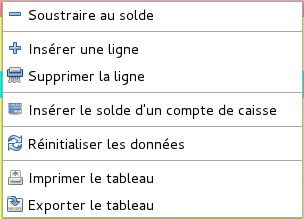
\includegraphics[scale=0.5]{image/screenshot/budget_estimate_context}}
% image entourée par une liste (picins)
\fi
	\item \menu{Soustraire au solde} ; 
	\item \menu{Ajouter au solde} ; 
	\item \menu{Insérer une ligne} ;
	\item \menu{Modifier la ligne} ;
	\item \menu{Supprimer la ligne} ;
	\item \menu{Supprimer toutes les occurrences de la ligne} ;
	\item \menu{Insérer le solde d'un compte de caisse} ;
	\item \menu{Convertir la ligne en opération planifiée} ;
	\item \menu{Réinitialiser les données} ;
	\item \menu{Imprimer le tableau} ;
	\item \menu{Exporter le tableau}.
\end{itemize}

% espace pour changement de thème
\vspacepdf{5mm}
Un \indexword{double-clic}\index{prévision !double-clic} sur une ligne d'opération du tableau ferme l'onglet \menu{Prévisions}, ouvre l'onglet \menu{Opérations}, sélectionne l'opération concernée et l'affiche dans le formulaire de saisie. De cette façon, cette opération peut être affichée et modifiée facilement.


\subsection{Graphiques sur les prévisions\label{budget-ertimate-chart}}

Pour afficher les \indexword{graphiques sur les prévisions}\index{prévision !graphiques} d'un compte, vous disposez de deux outils dans la barre d'outils :

\begin{itemize}
	\item \menu{Ligne} ou \menu{Colonne} : affiche un graphique temporel, pour l'évolution du montant du \menu{Solde} du compte ; 
	\item une liste déroulante : permet de choisir le graphique par défaut \menu{Ligne} ou \menu{Colonne}.
\end{itemize}

Ces graphiques fournissent une représentation visuelle de l'évolution future du solde du compte, et permettent d'en anticiper les conséquences par des mesures appropriées.


\subsubsection{Mode graphique ligne}

Pour afficher ce graphique, cliquez dans la barre d'outils sur l'outil \menu{Ligne} ou sur le libellé \menu{Ligne} de la liste déroulante ; une fenêtre affiche dans son onglet \menu{Graphique} la courbe d'évolution de la prévision du \menu{Solde} du compte, en fonction de la date sur la \menu{Durée d'estimation}. Vous pouvez afficher des lignes de niveau en cliquant sur le bouton \menu{Montrer la grille}, et les enlever par le bouton \menu{Cacher la grille}. 

Vous pouvez définir, dans l'onglet \menu{Options}, la présentation du graphique pour l'axe horizontal (graduation principale, position, ligne supplémentaire, orientation) et pour l'axe vertical (grille principale et secondaire). 


\subsubsection{Mode graphique colonne}

Pour afficher ce graphique, cliquez dans la barre d'outils sur l'outil \menu{Colonne} ou sur le libellé \menu{Colonne} de la liste déroulante ; une fenêtre affiche dans son onglet \menu{Graphique} l'évolution de la prévision du \menu{Solde} du compte, sous forme de barres verticales, en fonction de la date sur la \menu{Durée d'estimation}. Vous pouvez afficher les lignes de niveau en cliquant sur le bouton \menu{Montrer la grille}, et les enlever par le bouton \menu{Cacher la grille}.

Vous pouvez définir, dans l'onglet \menu{Options}, la présentation du graphique pour l'axe horizontal (graduation principale, position, ligne supplémentaire, orientation) et pour l'axe vertical (grille principale et secondaire), ainsi que pour les barres (espacement et superposition de la grille).


\section{Tableau d'amortissement\label{budget-amortization}}


Vous pouvez créer des tableaux d'amortissement afin de faire le suivi de vos \indexword{emprunts}\index{emprunt}. Les emprunts sont gérés dans Grisbi à l'intérieur de \indexword{comptes de passif}\index{compte !passif} (voir la section \vref{accounts-type-liabilities}, \menu{Type compte de passif}), à raison d'un seul emprunt par compte de passif, qu'il faudra que vous ayez créé auparavant. 

% espace pour changement de thème
\vspacepdf{5mm}
Pour afficher les détails du \menu{Tableau d'amortissement}, sélectionnez son onglet. Il affiche trois \ifIllustration éléments\refimage{budget-amortization-img} : 
\else éléments : 
\fi

\begin{itemize}
	\item la barre d'outils ;
	\item les données du crédit ; 
	\item le tableau d'amortissement détaillé.
\end{itemize} 

\ifIllustration
% image centrée 
\begin{figure}[t]
\begin{center}
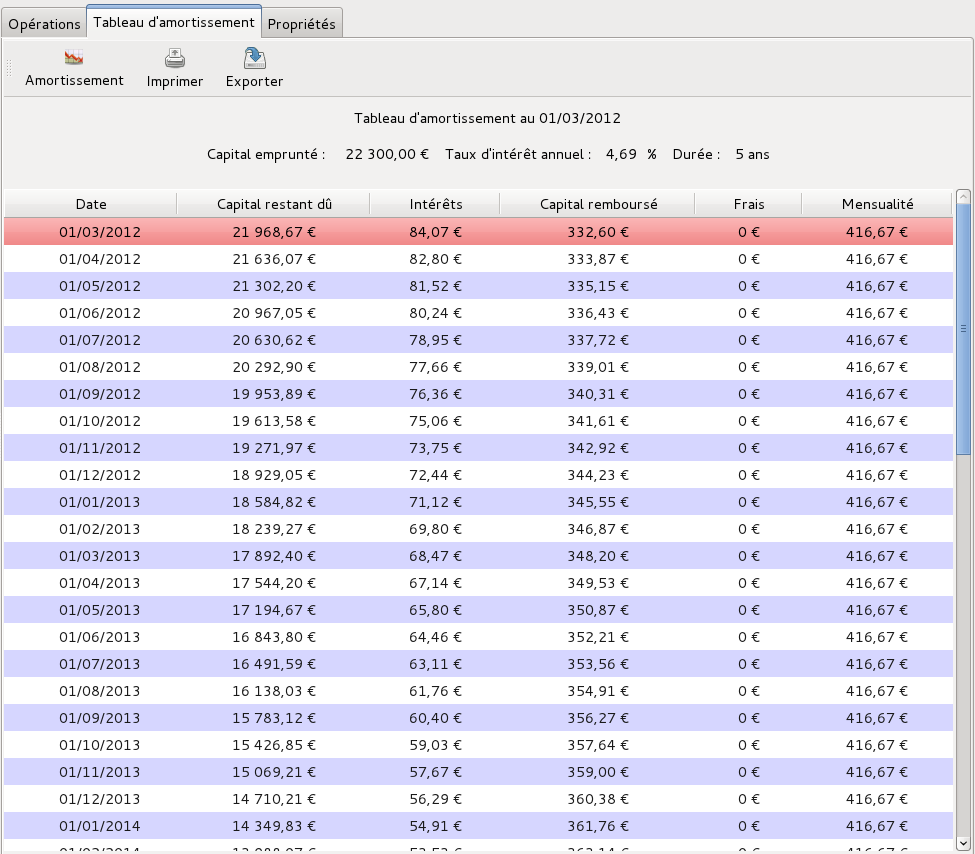
\includegraphics[scale=0.5]{image/screenshot/budget_amortization}
\end{center}
\caption{Tableau d'amortissement}
\label{budget-amortization-img}
\end{figure}
% image centrée
\fi

\ifIllustration
% saut de page pour paragraphe solidaire
\newpage
\fi


\subsection{Barre d'outils\label{budget-amortization-functions}}

La barre d'outils présente les fonctions suivantes  : 

\begin{itemize}
	 \item \menu{Depuis le début} ou \menu{À aujourd'hui} : affiche le tableau d'amortissement soit depuis le début du crédit, soit à partir de la prochaine échéance ;
	 \item \menu{Imprimer} : ouvre la fenêtre de sélection de l'imprimante et de ses options ;
	 \item \menu{Exporter} : permet d'exporter le tableau d'amortissement dans un fichier.
\end{itemize}


\subsection{Données du crédit\label{budget-amortization-data}}

Les données du crédit s'affichent en haut du pavé des détails, sous la barre d'outils. Elles affichent les paramètres tels qu'ils ont été définis auparavant, en particulier dans le menu \menu{Édition - Préférences} (voir la section \vref{setup-budget-data}, \menu{Données des comptes}). Ces paramètres sont les suivants :

\begin{itemize}
	 \item le \indexword{titre du tableau d'amortissement}\index{titre !tableau d'amortissement} : \menu{Tableau d'amortissement\ldots{ }}, suivi de la date, soit du début du crédit, soit de la prochaine échéance, en fonction de ce qui a été choisi par la fonction \menu{Depuis le début} ou \menu{À aujourd'hui} de la barre d'outils ;
	 \item le \menu{Capital emprunté} ; 
	 \item le \menu{Taux d'intérêt annuel} ;
	 \item la \menu{Durée du crédit}.
\end{itemize}


\subsection{Tableau d'amortissement détaillé\label{budget-amortization-table}}

Le tableau d'amortissement détaillé s'affiche en bas du pavé des détails, sous les données du \ifIllustration crédit\refimage{budget-amortization-img}.
\else crédit.
\fi
 Il affiche les caractéristiques détaillées de chaque échéance du crédit dont les paramètres sont affichés dans les données du crédit.

% espace pour changement de thème
\vspacepdf{5mm}
Il affiche en haut la barre de libellés des colonnes. Vous pouvez \indexword{élargir ou rétrécir une colonne}\index{colonne !largeur} en cliquant sur le séparateur entre deux colonnes et en le déplaçant. 

%XXXXXX Ne fonctionne pas  : XXXXXX Pour rétablir la largeur des colonnes à leur valeur par défaut, sélectionnez le menu \menu{Affichage - Réinitialiser la largeur des colonnes}. XXXXXX Ne fonctionne pas  : XXXXXX

% espace pour changement de thème
\vspacepdf{5mm}
Le tableau d'amortissement affiche autant de lignes qu'il y a d'échéances dans le crédit. Ses champs d'affichage sont les suivants :

\begin{itemize}
	 \item \menu{Date de l'échéance} ;
	 \item \menu{Capital restant dû} ;
	 \item \menu{Intérêts} ;
	 \item \menu{Capital remboursé} ;
	 \item \menu{Frais} ;
	 \item \menu{Mensualité}.
\end{itemize}

% espace pour changement de thème
\vspacepdf{5mm}
Vous pouvez déplacer la liste des échéances vers le haut ou vers le bas avec la molette de la souris, ou bien avec la souris et l'ascenseur vertical. 

%XXXXXX Ne fonctionne pas  : XXXXXX
%Le déplacement vers la gauche ou la droite se fait avec la souris et l'ascenseur horizontal.
%XXXXXX Ne fonctionne pas  : XXXXXX

Chaque échéance est affichée sur une ligne. Pour une bonne lisibilité de l'affichage, Grisbi présente une alternance de couleurs de fond violet et blanc{\couleurs} à chaque ligne.

% espace pour changement de thème
\vspacepdf{5mm}
Pour sélectionner une échéance, vous avez deux moyens :
\begin{itemize}
	 \item cliquer sur une de ses lignes ;
	 \item déplacer la sélection avec les touches du clavier \key{Flèche Haut}, \key{Flèche Bas}, \key{Page Haut}et \key{Page Bas}.
\end{itemize}
La ligne apparaît alors sur fond rouge{\couleur}.

% espace pour changement de thème
\vspacepdf{5mm}
Un menu contextuel est disponible par un clic-droit sur une ligne, et propose les actions suivantes :

\begin{itemize}
	 \item \menu{Afficher le tableau d'amortissement depuis le début}, si vous aviez choisi de l'afficher à partir de ce jour par la fonction  \menu{À aujourd'hui} de la barre d'outils ;
	 \item \menu{Afficher le tableau d'amortissement à ce jour}, si vous aviez choisi de l'afficher depuis le début du crédit par la fonction \menu{Depuis le début} de la barre d'outils ;
	 \item \menu{Imprimer le tableau} ;
	 \item \menu{Exporter le tableau}.
\end{itemize}


\section{Création d'un budget prévisionnel\label{budget-create}}


La création d'un budget prévisionnel pour un compte comprend quatre étapes :

\begin{enumerate}
	\item la configuration générale des budgets, si elle n'a pas déjà été faite auparavant ;
	\item la validation et la configuration du budget prévisionnel pour ce compte ;
	\item la sélection des données historiques de ce compte ;
	\item l'ajustement des prévisions.
\end{enumerate}

Le principe est, après avoir réalisé toutes les configurations, de sélectionner une par une, dans le \menu{Tableau des données historiques}, les lignes qui correspondent à des opérations qui vont normalement se reproduire dans le futur (par ex. Alimentation, Impôts, Assurances, Énergies, Salaire, etc.) ; ces choix se répercutent automatiquement dans le tableau des prévisions ; ensuite, dans l'onglet \menu{Prévisions}, d'ajuster le résultat en ajoutant de nouvelles opérations ou en supprimant celles inutiles. On peut cependant modifier à tout moment les choix opérés dans ce \menu{Tableau des données historiques}.

% espace pour changement de thème
\vspacepdf{5mm}
Les quatre étapes de création d'un budget prévisionnel sont décrites dans les sous-sections ci-dessous.


\subsection{Configuration générale des budgets\label{budget-create-general}}

Les paramètres généraux pour l'ensemble de vos budgets se trouvent dans le menu \menu{Édition - Préférences} (voir la section \vref{setup-budget-general}, \menu{Généralités}). Définissez là ces paramètres, si cela n'a pas déjà été fait auparavant, puis revenez à la sous-section ci-dessous.


\subsection{Validation et configuration d'un budget prévisionnel\label{budget-create-configure}}

Vous pouvez valider le budget prévisionnel pour un compte et configurer tous les paramètres dans le menu \menu{Édition - Préférences} (voir la section \vref{setup-budget-data}, \menu{Données des comptes}). 


\subsection{Sélection des données historiques\label{budget-create-selection}}

Pour afficher les détails des \menu{Données historiques}, sélectionnez leur onglet dans le compte concerné.

% espace pour changement de thème
\vspacepdf{5mm}
Dans l'\menu{En-tête des données historiques}, modifiez, si nécessaire, la source des données pour le compte ainsi que la période de référence pour ces données.

\textbf{Note} : le choix des exercices ne s'affiche que si au moins un exercice a été défini (voir la section \vref{financialyear-start}, \menu{Mise en place des exercices}).

Dans le \menu{Tableau des données historiques}, sélectionnez la première ligne : elle s'affiche sur fond rouge{\couleur} ; puis procédez comme suit :

\begin{enumerate}
	\item cochez la case à gauche de la ligne si elle correspond à des opérations récurrentes et que vous voulez la prendre comme référence : le champ \menu{Montant retenu} devient égal au champ \menu{Moyenne} ;
	\item déroulez cette ligne (petit triangle à gauche) : ses sous-catégories (ou sous-imputations budgétaires) s'affichent, toutes cochées, et la somme des montants retenus de ces sous-catégories est égal au montant retenu de la catégorie ;

	\textbf{Note} : ces triangles peuvent être remplacés, en fonction du thème de l'environnement de bureau ou du gestionnaire de fenêtres que vous utilisez, par d'autres caractères tels que +, -, >, <, etc.
	
	\item décochez les lignes de sous-catégorie (ou sous-imputation) qui ne sont pas récurrentes, qui sont donc occasionnelles ou imprévisibles, et que vous ne voulez pas prendre comme référence : le montant retenu de la catégorie devient nul (sa ligne est décochée automatiquement), et seuls restent les montants retenus des sous-catégories (ou sous-imputations) ;
	\item pour les lignes cochées, donc récurrentes, choisissez, grâce au menu contextuel, si vous voulez soit \menu{Copier la valeur moyenne} dans  le champ \menu{Montant retenu}, soit lui \menu{Assigner la valeur de la dernière opération}. 

	\textbf{Note} :	vous pouvez aussi forcer directement un montant dans ce champ : saisissez-le et validez-le par la touche \key{Entrée}.
\end{enumerate}

Exécutez cette procédure pour toutes les lignes suivantes de catégories (ou d'imputations budgétaires). Quand vous avez terminé toutes les lignes, vos données historiques sont supposées correctes et votre prévision sera calculée, au moins, par extrapolation de ces données. 

% espace pour changement de thème
\vspacepdf{5mm}
Sélectionnez maintenant l'onglet \menu{Prévisions} en cliquant dessus.


\subsection{Ajustement des prévisions\label{budget-create-adjust}}

Pour afficher les détails des \menu{Prévisions}, sélectionnez leur onglet  dans le compte concerné.

\textbf{Note} : pour les comptes de caisse, l'onglet \menu{Prévisions} n'est affiché  que si l'on a choisi de valider l'affichage de leurs prévisions (voir la section \vref{setup-budget-general}, \menu{Généralités}).
% espace après Attention ou Note  : 5 mm
\vspacepdf{5mm}

Dans l'\menu{En-tête des prévisions}, modifiez, si nécessaire, la \menu{Durée d'estimation}, la \menu{Date de départ} et la case à cocher \menu{Automatique} (info-bulle : \og \menu{Cochez la case pour changer automatiquement de date de début}\fg{}). 

% espace avant Attention ou Note  : 5 mm
\vspacepdf{5mm}
\textbf{Note} : la \indexword{date de début de prévision}\index{date !début de prévision} devrait être postérieure à aujourd'hui ; si vous saisissez une date de début de prévision antérieure, les prévisions inclueront toutes les opérations déjà enregistrées entre cette date et aujourd'hui.

% espace pour changement de thème
\vspacepdf{5mm}
Que la date de début de prévision soit antérieure ou postérieure à aujourd'hui, si vous cochez la case \menu{Automatique}, Grisbi  mettra automatiquement, à chaque ouverture du fichier de comptes, le début de la période de prévisions au premier jour du mois en cours. Par exemple, si la date de départ est le 1\up{er} janvier 2013 et la durée d'estimation 3 mois, vos prévisions commenceront ce jour-là et se termineront le 31 mars 2013 ; le jour du 1\up{er} février, les prévisions vont alors automatiquement commencer le 1\up{er} février et se terminer le 30 avril. Par contre, si la case n'avait pas été cochée, les prévisions auraient toujours commencé le 1\up{er} janvier et se seraient toujours terminées le 31 mars. 

% espace pour changement de thème
\vspacepdf{5mm}
Vous pouvez alors procéder au réglage fin de vos prévisions : dans le \menu{Tableau des prévisions}, un clic-droit sur une ligne, déjà sélectionnée ou non, l'affiche sur fond rouge{\couleur} avec un menu contextuel où vous pouvez sélectionner les actions suivantes :

\paragraph{Soustraire au solde :}la ligne sélectionnée reste affichée, mais le solde n'en tient plus compte.
 
\paragraph{Ajouter au solde :}la ligne sélectionnée reste affichée, mais le solde en tient compte à nouveau.

\paragraph{Insérer une ligne :}le formulaire de saisie \ifIllustration s'affiche\refimage{budget-insertLine-img}. Saisissez-y les champs d'une nouvelle opération, récurrente ou non, puis validez : l'opération s'affiche sur fond vert{\couleur}. On peut insérer une pseudo-opération planifiée, mais aussi un pseudo-virement, en choisissant comme catégorie un virement vers un autre compte. La \indexword{contre-opération}\index{contre-opération} de ce virement est automatiquement affichée dans l'onglet \menu{Prévisions} (s'il existe) du compte concerné, avec un montant inversé.
\else s'affiche. Saisissez-y les champs d'une nouvelle opération, récurrente ou non, puis validez : l'opération s'affiche sur fond vert{\couleur}. On peut insérer une pseudo-opération planifiée, mais aussi un pseudo-virement, en choisissant comme catégorie un virement vers un autre compte. La \indexword{contre-opération}\index{contre-opération} de ce virement est automatiquement affichée dans l'onglet \menu{Prévisions} (s'il existe) du compte concerné, avec un montant inversé.
\fi

\ifIllustration
% image centrée
\begin{figure}[htbp]
\begin{center}
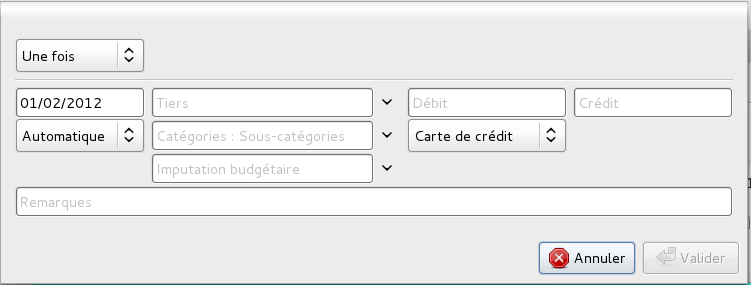
\includegraphics[scale=0.5]{image/screenshot/budget_insert_line}
\end{center}
\caption{Formulaire d'insertion d'une ligne}
\label{budget-insertLine-img}
\end{figure}
% image centrée
\fi

\paragraph{Modifier la ligne :}le formulaire de saisie s'affiche avec les paramètres de la ligne sélectionnée ; modifiez-y les champs de l'opération, puis validez : l'opération s'affiche sur fond vert{\couleur}. Certains champs peuvent ne pas être modifiables, donc si besoin est, il faut supprimer cette ligne et en insérer une nouvelle. Cette fonction ne peut apparaître que si vous aviez auparavant créé cette ligne par la fonction \menu{Insérer une ligne}.

\paragraph{Supprimer la ligne :}l'opération est supprimée, sans autre avertissement.

\textbf{Note} : il n'est pas possible de supprimer ici une ligne de prévision issue d'une opération planifiée ; cela doit être fait dans l'onglet \menu{Échéancier} (voir la section \ref{plannedtransactions-remove}, \menu{Suppression d'une opération planifiée}).

\paragraph{Supprimer toutes les occurrences de la ligne :}toutes les lignes d'une opération récurrente sont supprimées.  Cette fonction ne peut apparaître que si vous aviez auparavant créé cette ligne par la fonction \menu{Insérer une ligne}. 

\textbf{Note} : il n'est pas possible de supprimer ici toutes les lignes de prévision issues d'une opération planifiée ; cela doit être fait dans l'onglet \menu{Échéancier} (voir la section \ref{plannedtransactions-remove}, \menu{Suppression d'une opération planifiée}).

\paragraph{Insérer le solde d'un compte à débit différé :}cette fonction ouvre la fenêtre \menu{Configuration d'un compte à débit différé}, qui sert à configurer les prévisions pour des cartes bancaires à débit différé ; cette configuration et l'utilisation de cette fonction sont décrites en détail dans la section \ref{bankcard-deferredCard}, \menu{Carte bancaire à débit différé}.

\paragraph{Convertir la ligne en opération planifiée :}affiche la liste des opérations planifiées de l'onglet \menu{Échéancier}, puis copie et affiche cette ligne d'opération dans la liste en mode édition (sur fond rouge{\couleur}), et affiche le formulaire de saisie ; complétez-le et saisissez les paramètres manquants, en particulier ceux de périodicité (voir la section \vref{plannedtransactions-form}, \menu{Formulaire de saisie des opérations planifiées}). Cette fonction ne peut apparaître que si vous aviez auparavant créé cette ligne par la fonction \menu{Insérer une ligne}.

\paragraph{Réinitialiser les données :}recalcule le tableau de prévisions.

\paragraph{Imprimer le tableau :}ouvre la fenêtre de sélection de l'imprimante et de ses options (voir la section \ref{budget-print}, \menu{Impression d'un tableau de données historiques, de prévisions ou d'amortissement}).

\paragraph{Exporter le tableau :}permet d'exporter le tableau de prévisions dans un fichier (voir la section \vref{budget-export}, \menu{Export d'un tableau de données historiques, de prévisions ou d'amortissement}).

% espace pour changement de thème
\vspacepdf{5mm}
\textbf{Note} : chaque action terminée sur une opération déclenche le recalcul du tableau. 


\section{Modification d'un budget prévisionnel\label{budget-modify}}


Pour modifier un budget prévisionnel, reprenez les étapes décrites dans la section \vref{budget-create}, \menu{Création d'un budget prévisionnel}. 


\section{Création d'un tableau d'amortissement\label{budget-amortizationCreate}}


Pour créer un tableau d'amortissement dans un compte de passif, procédez comme suit :

\begin{enumerate}
	\item dans le menu \menu{Édition - Préférences}, sélectionnez \menu{Données des comptes} (voir la section \vref{setup-budget-data}, \menu{Données des comptes}) ;
	\item dans la liste déroulante, choisissez le compte de passif pour lequel vous voulez établir un tableau d'amortissement ;
	\item validez la case à cocher \menu{Utiliser le module budgétaire} : la zone \menu{Données du crédit} s'affiche ;
	\item saisissez les paramètres de votre crédit dans les cinq champs affichés ;
	\item choisissez le \menu{Type de taux} grâce à l'un des deux boutons \menu{Taux actuariel} ou \menu{Taux proportionnel} ;
	\item validez par le bouton \menu{Appliquer}, puis fermez la fenêtre par le bouton \menu{Fermer}.
\end{enumerate}

Dans le compte de passif concerné, un nouvel onglet \menu{Tableau d'amortissement} s'affiche entre les deux autres onglets \menu{Opérations} et \menu{Propriétés}, et le tableau d'amortissement est créé. Vous pouvez y afficher le tableau d'amortissement à partir de la date de début ou de la prochaine échéance par la fonction \menu{Depuis le début} ou \menu{À aujourd'hui} de la barre d'outils.


\section{Suppression d'un tableau de données historiques, de prévisions ou d'amortissement\label{budget-remove}}


Pour supprimer un tableau de données historiques, de prévisions ou d'amortissement sur un compte, il faut enlever les onglets \menu{Données historiques} et \menu{Prévisions}, ou l'onglet \menu{Tableau d'amortissement} ; procédez comme suit :


\begin{enumerate}
	\item dans le menu \menu{Édition - Préférences - Budget Prévisionnel - Données des comptes}, sélectionnez ce compte dans la liste déroulante ;
	\item décochez la case \menu{Utiliser le module budgétaire} : les zones en-dessous ne s'affichent plus ;
	\item cliquez sur le bouton \menu{Fermer}.	
\end{enumerate}

Dans le compte concerné, les onglets \menu{Données historiques} et \menu{Prévisions}, ou l'onglet \menu{Tableau d'amortissement}, ne s'affichent plus.

% espace avant Attention ou Note  : 5 mm
\vspacepdf{5mm}
\strong{Attention} : cette suppression ne supprime pas tout de suite les onglets, et vous pouvez les retrouver en revalidant le module budgétaire. Par contre, il sont totalement supprimés si vous enregistrez le fichier de comptes, ou si vous quittez Grisbi en enregistrant avant de quitter.


\section{Export d'un tableau de données historiques, de prévisions ou d'amortissement\label{budget-export}}


Grisbi vous permet d'exporter ces tableaux, soit pour les enregistrer, soit pour les importer dans une autre application, par exemple un tableur pour y faire des calculs spécifiques. 

% espace pour changement de thème
\vspacepdf{5mm}
Pour exporter un tableau de données historiques, de prévisions ou d'amortissement, procédez comme suit :
\begin{enumerate}
	 \item dans l'onglet \menu{Prévisions} ou \menu{Tableau d'amortissement}, cliquez sur l'outil \menu{Exporter} dans la barre d'outils ; ou bien cliquez-droit sur une des lignes du tableau, puis sélectionnez \menu{Exporter le tableau} dans le menu contextuel ; une fenêtre de gestionnaire de fichiers s'affiche ;
	 \item saisissez le nom du fichier à exporter, dont l'\indexword{extension} sera \file{.csv}\index{extension !.csv} ;
	 \item choisissez son répertoire de destination ;
	 \item cliquez sur le bouton \menu{Enregistrer}.
\end{enumerate}

% espace avant Attention ou Note  : 5 mm
\vspacepdf{5mm}
\strong{Attention} : d'une manière générale, il est déconseillé d'avoir des accents ou des espaces dans les noms des répertoires et fichiers utilisés par Grisbi. Si c'est le cas, renommez-les maintenant. Par exemple, les espaces peuvent être remplacées par des tirets bas (\_). 


\section{Impression d'un tableau de données historiques, de prévisions ou d'amortissement\label{budget-print}}

Pour imprimer un tableau de données historiques, de prévisions ou d'amortissement, procédez comme suit :

\begin{enumerate}
	 \item dans l'onglet \menu{Données historiques}, \menu{Prévisions} ou \menu{Tableau d'amortissement}, cliquez sur le bouton \menu{Imprimer} de la barre d'outils, ou bien cliquez-droit sur une des lignes du tableau puis sélectionnez \menu{Imprimer le tableau} dans le menu contextuel ;
	 \item  une fenêtre d'impression s'ouvre, dont l'aspect et les fonctions dépendent de votre gestionnaire d'impression ; vous aurez le plus souvent les choix suivants :
		  \begin{itemize}
			  \item imprimer dans un fichier (au format \indexword{\gls{PostScript}}\index{postscript}, \indexword{\gls{PDF}}\index{pdf} ou \indexword{\gls{SVG}}\index{svg}),
			  \item imprimer avec votre imprimante.
		  \end{itemize}
\end{enumerate}

En fonction de votre gestionnaire d'impression, vous pourrez disposer de réglages divers tels que la taille et l'orientation de la feuille, la résolution, la police d'impression et sa taille, etc.

% espace avant Attention ou Note  : 5 mm
\vspacepdf{5mm}
\textbf{Note} : un tableau de données historiques, de prévisions ou d'amortissement peut être très long ; affichez un aperçu avant impression pour vérifier ce que vous allez imprimer.



